\documentclass[10pt,letterpaper]{article}
\usepackage[T1]{fontenc}
\usepackage[utf8]{inputenc}
\usepackage{lmodern}
\usepackage[margin=0.9in]{geometry}
\usepackage{graphicx}
\usepackage[table,dvipsnames]{xcolor}
\usepackage{colortbl}
\usepackage{array}
\usepackage{booktabs}
\usepackage{float}
\usepackage{caption}
\usepackage{enumitem}
\usepackage{amsmath}
\usepackage{fancyhdr}
\usepackage{titlesec}
\usepackage{microtype}
\usepackage[hidelinks]{hyperref}

\definecolor{navy}{HTML}{1F3A5F}
\definecolor{teal}{HTML}{2A9D8F}
\definecolor{grey}{HTML}{8D99AE}

\setlist[itemize]{leftmargin=1.3em,itemsep=1pt,topsep=2pt}
\titleformat{\section}{\Large\bfseries\color{navy}}{\thesection}{0.6em}{}
\titleformat{\subsection}{\large\bfseries\color{navy}}{\thesubsection}{0.6em}{}
\titlespacing*{\section}{0pt}{14pt}{6pt}
\titlespacing*{\subsection}{0pt}{10pt}{4pt}
\captionsetup{font=small,labelfont=bf,justification=raggedright,singlelinecheck=false}
\setlength{\parindent}{0pt}
\setlength{\parskip}{4pt}

\newcommand{\good}{\textcolor{teal}{\textbf{Selected}}}
\newcommand{\methodrow}[3]{\textbf{#1} & #2 & #3 \\}

\pagestyle{fancy}
\fancyhf{}
\renewcommand{\headrulewidth}{0.4pt}
\fancyhead[L]{\small\textcolor{navy}{Capitolis CCR Engine -- Methods, Results \& Trade-offs}}
\fancyhead[R]{\small\textcolor{navy}{\thepage}}

\title{\textcolor{navy}{\textbf{Counterparty Credit Risk Engine}}\\[4pt]
\Large Methods, Trade-offs, and Results}
\author{Berkeley MFE Industry Project -- Capitolis}
\date{\today}

\begin{document}
\maketitle
\thispagestyle{fancy}

\section*{Executive Summary}
This memo documents every material design decision behind the Monte Carlo counterparty credit risk engine built for Capitolis' 16-trade ESF book: the alternatives considered at each stage, the quantitative trade-off between them, and why the selected approach won. It intentionally omits standard definitions (CVA, PFE, Hull-White, etc. -- covered in the 77-page technical report) and instead states, stage by stage: \emph{what we tried, what it cost or gained, and what we concluded.}

\begin{center}
\small
\begin{tabular}{lrr}
\toprule
& \textbf{Close-out (brief's definition)} & \textbf{Level (uncollateralized)} \\
\midrule
Portfolio MPE99 & \$51.0M & \$201.9M \\
CVA / SA-CVA capital & \$11.7k / \$0.10M & \$247k / \$2.23M \\
KVA (10\% cost of capital) & \$22.4k & \$470k \\
\bottomrule
\end{tabular}
\end{center}

\section{Risk-Factor Models: One Choice at Each Layer}

\subsection{USD interest rates: one-factor vs.\ two-factor Hull-White}
\textbf{Alternatives considered.} A one-factor Hull-White model (single Gaussian short-rate factor, mean-reverting) versus a two-factor extension, G2++, equivalent to a two-factor LGM, in which a second correlated factor lets the curve twist rather than only shift in parallel.

\textbf{Method.} Both were fully implemented and calibrated to real data: the one-factor model's mean reversion ($a=0.0167$) from the real USD swaption ATM normal-vol cube, its volatility (0.96\%) from realised 2y--30y Treasury yield changes; the two-factor model's five parameters fitted by least squares to the realised covariance of those same yields.

\begin{center}\small
\begin{tabular}{p{0.32\textwidth}p{0.22\textwidth}p{0.38\textwidth}}
\toprule
& \textbf{One-factor HW} & \textbf{Two-factor G2++} \\
\midrule
Fit to realised yield covariance & -- & 16.1\% relative error \\
Parameters at a bound & no & $b=1.5$ (upper bound), $\rho=-0.95$ \\
Effect on portfolio MPE99 & baseline & $-3.0\%$ (A $-1\%$, B $-3\%$, C $-0\%$) \\
\bottomrule
\end{tabular}
\end{center}

\textbf{Conclusion: one-factor selected as the production default.} The two-factor fit strains to match a hump-shaped realised vol curve it cannot fully represent (Figure~\ref{fig:g2fit}), and even a successful fit moves the headline number by only 3\%. The book's dominant rate exposure is one large short forward on a single long bond -- a level bet, not a curve-shape bet -- so the extra parameters buy little. G2++ is retained as a documented, validated comparison, not a production choice; the natural next step, if adopted, is calibrating it to the swaption cube rather than realised yields.

\begin{figure}[H]
\centering
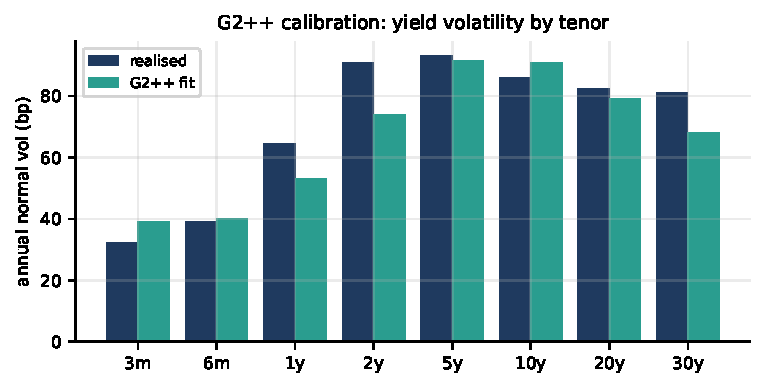
\includegraphics[width=0.85\linewidth]{figures/fig19.pdf}
\caption{Realised yield-change volatility by tenor against the fitted two-factor model. The one-factor model's single decaying exponential cannot reproduce this hump either, but changes the headline number far less than the fitting effort would suggest.}
\label{fig:g2fit}
\end{figure}

\subsection{JPY rates: a second, independent Hull-White factor vs.\ a constant differential}
\textbf{Alternatives considered.} (i) No JPY rate factor: JPY-listed names and USDJPY drift off a single constant USD--JPY rate differential backed out from market data; (ii) a genuine second, simulated Hull-White factor for JPY, built from the real JPY OIS curve.

\textbf{Trade-off.} The constant-differential approach is materially cheaper (no extra factor to simulate or correlate) but cannot represent JPY rate risk moving independently of USD rates, and cannot represent negative JPY rates, which have been the norm for most of the last 25 years (Figure~\ref{fig:tona}).

\textbf{Result.} Adding the JPY factor moved the portfolio MPE99 attribution from \$52.1M to \$51.5M (Section~\ref{sec:attribution}) -- a real, disclosed effect, not noise. The Gaussian model natively supports negative rates with no floor, validated on a synthetic negative curve (63\% of simulated points negative, nothing clipped).

\textbf{Conclusion: JPY factor selected.} Two of the eight equity swaps are JPY-compo trades and USDJPY itself is a risk factor for both bond trades' funding legs; a constant differential would silently misstate their risk whenever JPY and USD policy diverge, which the data show they do (day-to-day rate changes are essentially uncorrelated at $-0.04$, despite yield \emph{levels} moving together at $\sim$0.38 with the global cycle).

\begin{figure}[H]
\centering
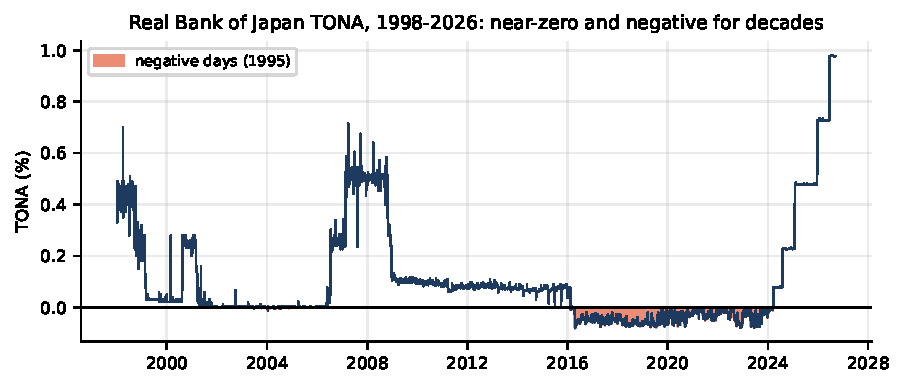
\includegraphics[width=0.75\linewidth]{figures/fig16.pdf}
\caption{Real Bank of Japan TONA history: negative or zero for most of 25 years. A model that floors at zero cannot represent this regime.}
\label{fig:tona}
\end{figure}

\subsection{Equity/FX correlation: full Cholesky matrix vs.\ PCA factor model}
\textbf{Alternatives considered.} Correlate the 39 factors' random draws using (i) the full $39\times39$ Cholesky-decomposed correlation matrix every scenario, or (ii) a reduced $k$-factor PCA representation (draw $k$ systematic factors plus idiosyncratic noise, cheaper in principle for large $k$-vs-$n$ problems).

\begin{center}\small
\begin{tabular}{lrrr}
\toprule
& \textbf{Full matrix} & \textbf{PCA, $k=5$} & \textbf{PCA, $k=10$} \\
\midrule
Correlated-shock step (5,000 scen.) & 1.91s & 2.08s & 2.29s \\
Variance explained & 100\% & 47\% & 62\% \\
Netting-set vol vs.\ full (CPTY\_B) & -- & $+1.7\%$ & $+0.5\%$ \\
\bottomrule
\end{tabular}
\end{center}

\textbf{Conclusion: full matrix selected; PCA kept only as an explainability tool.} At $n=39$ the reduced representation is \emph{slower}, not faster, because it draws $k$ systematic plus $n$ idiosyncratic random numbers instead of $n$ correlated ones directly -- there is no dimensionality win at this scale. PCA remains useful for describing \emph{what} the 39 names have in common (a market factor, a Japan-vs-US factor, etc., Figure~\ref{fig:pca}), not for speed.

\begin{figure}[H]
\centering
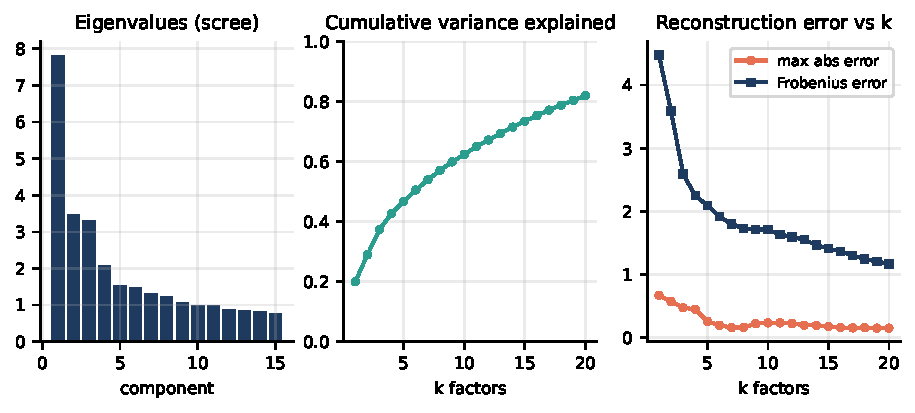
\includegraphics[width=0.95\linewidth]{figures/fig14.pdf}
\caption{Eigenvalue scree, cumulative variance explained, and reconstruction error vs.\ $k$. Five factors explain 47\% of variance; ten explain 62\%.}
\label{fig:pca}
\end{figure}

\section{Calibration: Choosing Between Real-Data Routes}

\subsection{Mean reversion ($a$): swaption-implied vs.\ futures-implied}
\begin{center}\small
\begin{tabular}{p{0.24\textwidth}p{0.34\textwidth}p{0.1\textwidth}p{0.2\textwidth}}
\toprule
\textbf{Route} & \textbf{Data} & \textbf{$a$ (USD)} & \textbf{Verdict} \\
\midrule
Swaption cube (preferred) & Bloomberg ATM normal vol, 1M expiry & 0.0167 & \good\ used \\
SOFR-futures vol decay & 2y Databento history & 0.0458 & cross-check only \\
\bottomrule
\end{tabular}
\end{center}
The two real-data routes disagree (different instruments, different tenor ranges) but both give sensible, positive values -- the swaption route is the textbook standard and was preferred. For JPY, all three real routes tried (swaption cube, JGB yield history, OIS history) return a \emph{negative} $a$, meaning JPY forward-rate volatility genuinely rises with tenor rather than decaying, so we use the lowest admissible value ($a=0.001$, the Ho-Lee limit) rather than an invalid fit.

\subsection{Rate volatility: realised long-end yield vol vs.\ realised overnight SOFR vol}
The original volatility source was the realised volatility of the overnight SOFR fixing itself (0.63\%). Overnight fixings move in discrete steps on Fed days and materially understate how far the \emph{long-dated} yields this book actually depends on move: the realised 10-day change of the 20-year yield has a standard deviation of about 15bp against roughly 11bp implied by the overnight-fixing sigma. Refitting sigma to the realised vol of 2y--30y Treasury yields (0.96\%) instead is a disclosed, deliberate change, confirmed by the Kupiec backtest (Section~\ref{sec:validation}) and reflected in the attribution table (Section~\ref{sec:attribution}, row 2).

\subsection{Implied vs.\ realised volatility: which is used where}
\begin{center}\small
\begin{tabular}{p{0.24\textwidth}p{0.24\textwidth}p{0.42\textwidth}}
\toprule
\textbf{Parameter} & \textbf{Source} & \textbf{Why} \\
\midrule
Rate mean reversion ($a$) & Real swaption cube (implied) & Standard route; decay shape is what implied vol reveals \\
Rate volatility ($\sigma$) & Realised long-end Treasury vol & Swaption fit is a simplified single-expiry read; realised level validated by backtest \\
Equity / FX volatility & Realised (3y history) & No implied-vol source available; disclosed proxy \\
JPY $\sigma$ (fallback path only) & Swaption vol level & No sufficiently long realised JPY history to fit against \\
\bottomrule
\end{tabular}
\end{center}

\section{Simulation Methodology}

\subsection{Sampling scheme: five methods compared}
\textbf{Alternatives.} Pseudo-random, antithetic pairing, moment-matching, Sobol quasi-random, and Latin Hypercube, tested on (i) a controlled European-call benchmark with a known Black-Scholes answer, and (ii) the real 663-dimensional engine (39 factors $\times$ 17 steps).

\begin{figure}[H]
\centering
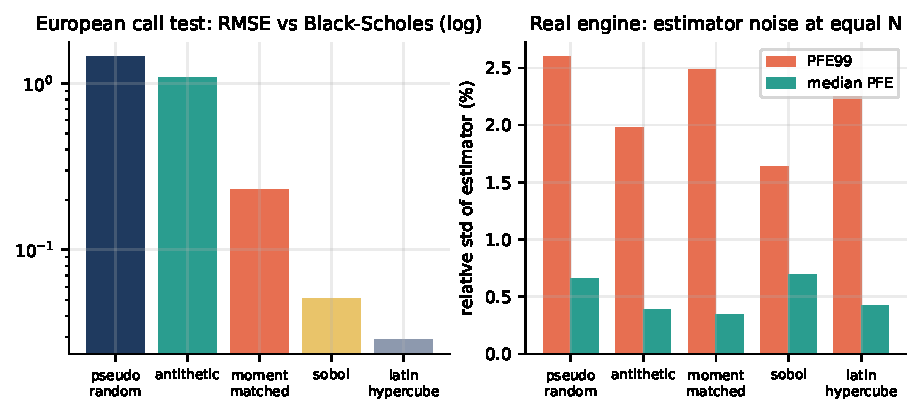
\includegraphics[width=0.95\linewidth]{figures/fig21.pdf}
\caption{Left: on the controlled benchmark, Latin Hypercube has $\sim$51x lower error than pseudo-random. Right: on the real engine the methods converge much closer, and no single method wins on both PFE99 and median PFE.}
\label{fig:sampling}
\end{figure}

\textbf{Conclusion: Latin Hypercube selected.} It is the only method that is simultaneously best on the controlled test and better than pseudo-random on both real-engine statistics, at negligible extra cost. Sobol is the runner-up on the controlled test but its advantage disappears for the median PFE at this dimensionality.

\subsection{Exposure convention: close-out (the brief) vs.\ uncollateralized level}
Both are computed throughout, on the same paths, because they answer different questions and neither alone is defensible without knowing the real margin terms:
\begin{center}\small
\begin{tabular}{lrr}
\toprule
& \textbf{Close-out} & \textbf{Level} \\
\midrule
Definition & $\max(V(t{+}10\text{bd})-V(t{-}1\text{bd}),0)$ & $\max(V(t),0)$ \\
Assumes & Daily VM, no IM/threshold & No margin at all \\
Portfolio MPE99 & \$51.0M & \$201.9M \\
\bottomrule
\end{tabular}
\end{center}
\textbf{Conclusion:} close-out is the brief's definition and the primary number throughout; level is reported as a no-margin upper bound, since the real CSA terms (threshold, MTA, IM) were not supplied.

\subsection{Scenario count: how many is enough}
Standard error was estimated by bootstrap resampling rather than rerunning the (expensive) full repricing at every candidate $N$.
\begin{center}\small
\begin{tabular}{p{0.08\textwidth}p{0.2\textwidth}p{0.16\textwidth}p{0.44\textwidth}}
\toprule
\textbf{$N$} & \textbf{Rel.\ SE, PFE99} & \textbf{Est.\ time (8 cores)} & \textbf{Use} \\
\midrule
1,000 & higher & $\sim$2 min & Iteration / what-if \\
5,000 & moderate & $\sim$8 min & \good\ Standard reporting \\
10,000 & lower & $\sim$15 min & Limit sign-off \\
15,000+ & diminishing returns & -- & Not recommended: cost scales linearly, error only as $1/\sqrt{N}$ \\
\bottomrule
\end{tabular}
\end{center}
Beyond $\sim$15,000 scenarios, the remaining sampling error is an order of magnitude smaller than the model-risk sensitivities in Section~\ref{sec:modelrisk} -- more scenarios stop being the binding constraint on precision well before that point.

\section{Sensitivities (Greeks): Methods Compared}

\subsection{Noise control: common random numbers}
Bumping a risk factor and repricing with \emph{independent} random draws produces an estimator with standard deviation \$245k; reusing the identical draws in the base and bumped run (common random numbers, CRN) cuts that to \$1k -- \textbf{282x lower}. Every Greek in this project uses CRN; this, not the sampling scheme, is what actually controls sensitivity noise (confirmed again in Section~\ref{sec:lhs-sampling-greeks}).

\subsection{Equity/FX bumps: exact path rescaling vs.\ naive resimulation}
Because equity and FX paths are geometric Brownian motion, a spot bump rescales every simulated path \emph{exactly} in closed form -- no resimulation needed.
\begin{center}\small
\begin{tabular}{lrr}
\toprule
& \textbf{Time (N=300, idle machine)} & \textbf{vs.\ naive} \\
\midrule
Base run & 105s & -- \\
78 equity/FX bumps (exact rescaling) & 88s & \textbf{93x cheaper} than naive \\
78 equity/FX bumps, naive resimulation (est.) & $\sim$8,166s & baseline \\
\bottomrule
\end{tabular}
\end{center}

\subsection{Pathwise (closed-form) delta vs.\ bump-and-reprice}
For linear (equity/FX) exposure, a pathwise estimator exists in closed form and needs no repricing at all.
\begin{center}\small
\begin{tabular}{lrr}
\toprule
& \textbf{Runtime} & \textbf{Agreement with bump-and-reprice} \\
\midrule
Bump-and-reprice (reference) & $\sim$260s & -- \\
Pathwise (closed-form) & 0.2--0.4s & median 0.02\%, worst 0.4\% (EE) \\
\bottomrule
\end{tabular}
\end{center}
\textbf{Conclusion:} pathwise is validated and $\sim$1000x faster for EE, but noisier for quantile Greeks (PFE99), so bump-and-reprice with CRN remains the reported figure; pathwise serves as the fast cross-check. Adjoint algorithmic differentiation was considered and rejected for this project: it would price all Greeks for the cost of $\sim$3--5 valuations, but requires the pricing library to be rewritten in differentiable form, which was out of scope.

\subsection{Rate/vol bumps: an exact method that reuses the same simulated draws}\label{sec:lhs-sampling-greeks}
\textbf{The insight.} In the one-factor Hull-White model, $r(t)=x(t)+\alpha(t)$, where $x(t)$ is the simulated stochastic factor and $\alpha(t)$ is a deterministic function of the curve, $a$ and $\sigma$ only. A curve bump that leaves $a,\sigma$ fixed (every DV01 bump here) leaves $x(t)$ \textbf{identical} to the base run. The entire effect on every equity/FX path is therefore one deterministic number per date, addable to the base run's own paths.

\textbf{Validation.} Compared against a true, independent resimulation of the bumped scenario: agreement to $10^{-15}$ relative precision -- the same calculation, not an approximation, computed without drawing any new randomness.

\textbf{Does Latin Hypercube itself reduce Greeks noise (a separate question)?} Tested directly: mixed. LHS cuts EE-delta noise 15--85\% but shows no consistent benefit -- sometimes markedly worse -- for tail-quantile (PFE99) deltas (Figure~\ref{fig:samplinggreeks}), because stratifying 663 marginal dimensions does not concentrate coverage on the handful of scenarios that set a 99th-percentile outcome.

\begin{figure}[H]
\centering
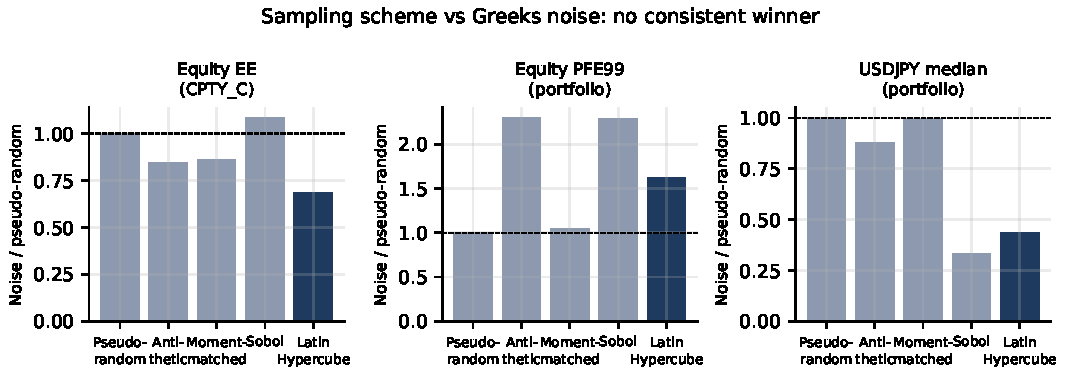
\includegraphics[width=0.95\linewidth]{figures/fig_sampling_greeks.pdf}
\caption{Standard deviation of each Greek across seeds, by sampling scheme, relative to pseudo-random. No scheme wins consistently.}
\label{fig:samplinggreeks}
\end{figure}

\section{Rate DV01: Two Independent Improvements}

\subsection{Zero-rate tenor grid vs.\ par-instrument (Jacobian) buckets}
\textbf{Alternatives.} (i) Bump the \emph{fitted} zero curve at 8 hand-chosen tenors with a triangular interpolation weight (original method); (ii) bump the curve's own $\sim$45 native construction pillars (SOFR-futures-implied points and every individual Bloomberg-spliced long-end point) directly, grouped into the same 8 report buckets by nearest pillar.

\begin{center}\small
\begin{tabular}{p{0.42\textwidth}p{0.24\textwidth}p{0.24\textwidth}}
\toprule
\textbf{Report bucket} & \textbf{Old (zero-grid)} & \textbf{New (par-instrument)} \\
\midrule
10y bucket, share of portfolio DV01 & 39\% & 11\% \\
30y bucket, share of portfolio DV01 & 54\% & \textbf{82\%} \\
\midrule
Bucket sum vs.\ independent parallel bump & within 0.1\% & within 0.1\% \\
\bottomrule
\end{tabular}
\end{center}

\begin{figure}[H]
\centering
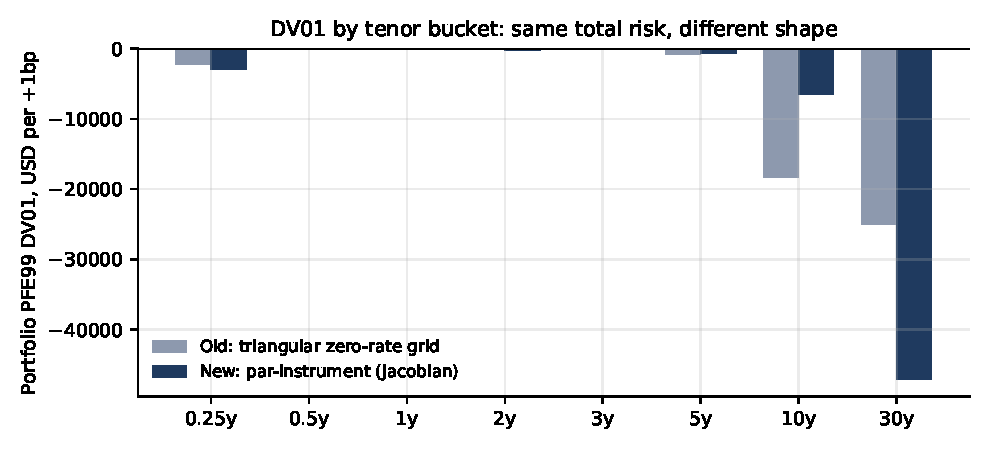
\includegraphics[width=0.7\linewidth]{figures/fig_dv01_compare.pdf}
\caption{Same total rate risk, different attribution across tenor.}
\label{fig:dv01}
\end{figure}

\textbf{Conclusion: par-instrument method selected as the primary DV01 breakdown.} Both methods sum to the same total (an internal consistency check), but the original grid was smearing risk that genuinely lives in the 20--50y region -- where BF\_0003, the dominant \$500M bond forward maturing 2049, sits -- partly into the 10y bucket. The par-instrument method is also the textbook definition of a Jacobian sensitivity: it ties the bump to the real, tradeable instruments the curve was built from, not an invented interpolation.

\subsection{Resimulated vs.\ exact-shift computation of the same buckets}
Applying the insight from Section~\ref{sec:lhs-sampling-greeks}, the 8 par-instrument buckets plus the parallel bump were computed with the exact analytic path-shift rather than resimulation: the whole computation pays the simulation cost once (the base run), not once per bucket, with no loss of accuracy (validated to $10^{-15}$ as above).

\section{Stress Testing Design}
\textbf{Method.} 13 fixed scenarios, each an instantaneous shock to today's market state followed by a full exposure re-run with the same random draws as the base case: 8 round-number (equities $\pm$30\%, yen $\pm$15\%, rates $\pm$200bp, flight-to-quality, stagflation) plus 5 historical replays, each chosen by an objective worst-window rule rather than by hand.

\textbf{Extension for this round of feedback.} The original 3 historical replays only covered 2014--2026 (the primary price-history window). Public price history was extended back to 2007 (28 of 37 names covered) to add two named episodes: the 2008 financial crisis (worst window found: Sep 29--Oct 10, 2008) and the August 2015 RMB devaluation.

\begin{center}\small
\begin{tabular}{lrr}
\toprule
\textbf{Scenario} & \textbf{Close-out MPE99} & \textbf{Level MPE99} \\
\midrule
2020 equity crash (existing) & $-15\%$ & $+55\%$ \\
\textbf{2008 GFC (new)} & $-13\%$ & $+56\%$ \\
\textbf{2015 China deval.\ (new)} & $-5\%$ & $+16\%$ \\
\bottomrule
\end{tabular}
\end{center}

\textbf{Conclusion:} the two new episodes land inside the range the existing scenarios already covered, not beyond it -- a validation finding, not just an added data point: the absence of a 2008 replay was not previously understating the tail.

\begin{figure}[H]
\centering
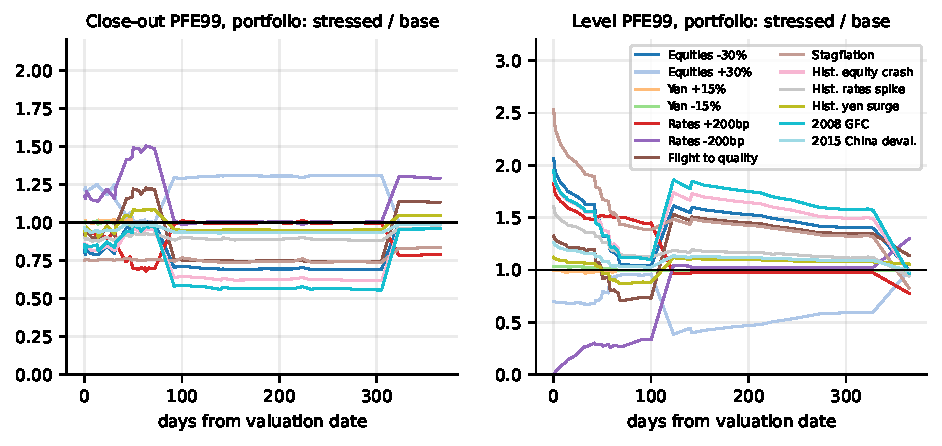
\includegraphics[width=0.85\linewidth]{figures/fig33.pdf}
\caption{Ratio of stressed to base portfolio PFE99 along the first year, close-out (left) and level (right) exposure.}
\label{fig:stress}
\end{figure}

\section{Credit and Capital: CVA, DVA, FVA, KVA}

\subsection{Credit-spread source: CDS vs.\ rating-based bond-index proxy}
No CDS quotes are available for the anonymised counterparties. Basel MAR50.32(3) explicitly permits proxying an illiquid name's spread by credit quality (rating), industry, and region; here, only credit quality is used (industry/region unknown), via ICE BofA US corporate OAS indices by rating (public, FRED). The maturity \emph{shape} is taken from the broad all-corporate index by bucket and applied to every rating -- a disclosed simplification, since the shape is not rating-specific. This same construction is reused for the extra-credit risky-bond sample trade's issuer curve.

\subsection{Exposure convention for CVA: close-out vs.\ level}
Both are computed. On close-out, positive and negative exposure are nearly symmetric (both are 10-day moves from a margined start), so CVA and DVA nearly cancel; on level, the asymmetry is large (the book is net in Capitolis' favour), so CVA and FCA dominate DVA and FBA.
\begin{center}\small
\begin{tabular}{lrrrr}
\toprule
& \textbf{CVA} & \textbf{DVA} & \textbf{FVA} & \textbf{KVA (10\% CoC)} \\
\midrule
Close-out & \$11.7k & \$11.2k & \$0.5k & \$22.4k \\
Level (uncollateralized) & \$247k & \$7.5k & \$240.0k & \$470k \\
\bottomrule
\end{tabular}
\end{center}

\subsection{KVA: capital-charge proxy, cost-of-capital swept, not assumed}
No capital methodology or Capitolis cost of capital was supplied, so $K(t)=8\%\times\text{RW}\times\alpha\times\text{EPE}(t)$ (Basel minimum ratio, standard SA-CCR $\alpha=1.4$) is discounted and integrated exactly like the other xVA terms, then scaled by a swept 8/10/12\% cost-of-capital grid rather than one assumed figure. KVA exceeds CVA on both conventions because it scales the entire EPE profile by a fixed ratio rather than a small investment-grade default probability -- explicitly illustrative pending a real methodology.

\section{Independent Validation}\label{sec:validation}
Four independent checks, each testing a different failure mode:
\begin{center}\small
\begin{tabular}{p{0.16\textwidth}p{0.24\textwidth}p{0.24\textwidth}p{0.24\textwidth}}
\toprule
\textbf{Check} & \textbf{Method} & \textbf{Result} & \textbf{Catches} \\
\midrule
Martingale test & Discounted asset paths should average to today's price & Pass & Drift / discretisation bugs \\
Parametric VaR benchmark & Delta-normal VaR vs.\ full MC P\&L & \$11.4M vs.\ \$11.7M (ratio 0.98) & Sign / scaling errors in deltas \\
Kupiec backtest (99\%) & Historical exceedances vs.\ 5,000-scenario prediction & 4 / 6 / 2 exceptions vs.\ 2.4 expected (all pass) & Miscalibrated tail \\
Excel parametric checks & Independent spreadsheet formulas on public data & 0.1--7\% agreement across 4 checks & Calibration \& simulation errors, no code trust needed \\
\bottomrule
\end{tabular}
\end{center}
The Excel workbook (\texttt{Capitolis\_CCR\_Parametric\_Benchmarks.xlsx}) independently recomputes calibrated volatilities from raw public prices with live spreadsheet formulas (\texttt{=STDEV(LN(Pt/Pt-1))*SQRT(252)}), matching the model to $\sim$0.1\%; compares the simulated one-year volatility to the closed-form $\text{vol}\times\sqrt{T}$ (1--2\% agreement); and compares a Monte Carlo equity vega against the closed-form Black vega under a $\pm1\%$ vol bump (7\% agreement).

\section{Model Risk: What Actually Moves the Number}\label{sec:modelrisk}
Each input perturbed one at a time, same scenario count, same random draws (base portfolio MPE99 = \$51.5M at $N{=}2{,}000$):
\begin{center}\small
\begin{tabular}{lr}
\toprule
\textbf{Perturbation} & \textbf{Change in portfolio MPE99} \\
\midrule
Equity/FX vol $\times2$ & $+71\%$ \\
Equity correlations, 30\% toward 1 & $+22\%$ \\
Equity/FX vol $\times1.25$ & $+19\%$ \\
Rate--equity dependence, both fall together & $+18\%$ \\
Rate volatility $\times1.25$ & $+9\%$ \\
Rate--equity dependence, offsetting & $-15\%$ \\
Mean reversion $a\times3$ & $-5\%$ \\
Two-factor rate model (G2++) instead of one-factor & $-3\%$ \\
\bottomrule
\end{tabular}
\end{center}
\textbf{Conclusion:} equity volatility and correlation, and the (data-unresolvable) sign of the rate--equity dependence, dominate model risk. The rate-model choice explored at length in Section~1.1 (one- vs.\ two-factor Hull-White) is, by comparison, one of the \emph{smallest} levers in the entire model -- which is itself the strongest argument for keeping the simpler model as the default.

\begin{figure}[H]
\centering
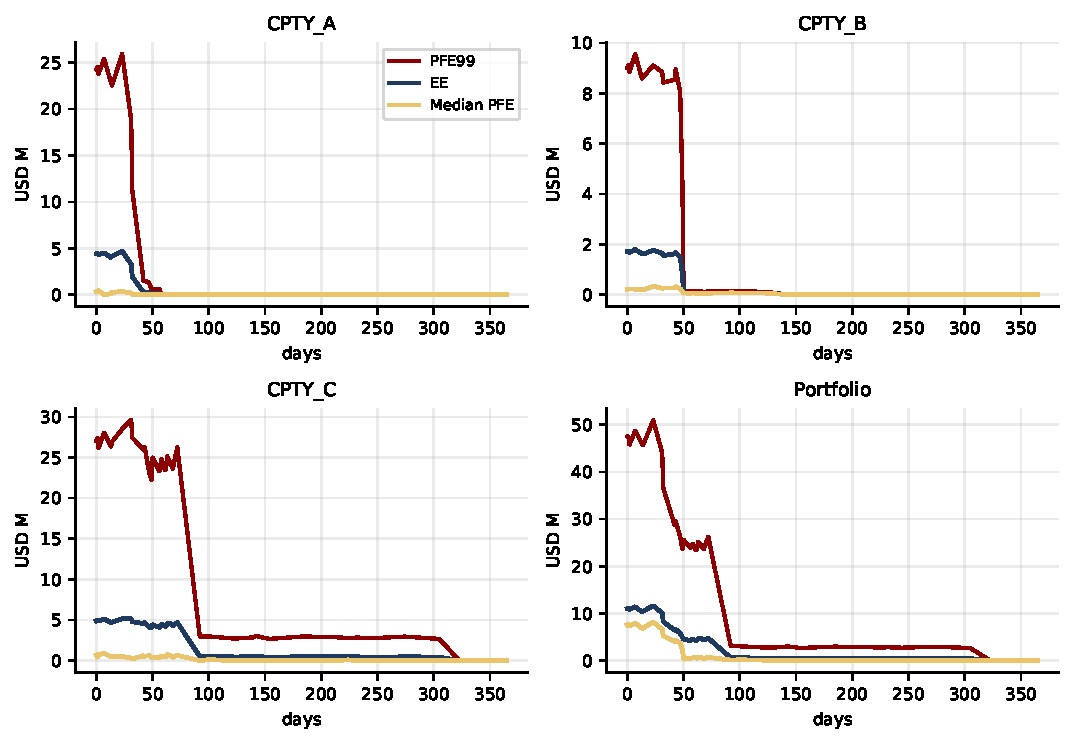
\includegraphics[width=0.7\linewidth]{figures/fig25.pdf}
\caption{Close-out exposure profile (EE, median PFE, PFE99) by counterparty and portfolio -- the baseline every trade-off in this memo is measured against.}
\label{fig:exposure}
\end{figure}

\section{Attribution: Every Correction, One at a Time}\label{sec:attribution}
Each fix introduced cumulatively on the same random numbers and scenario count, portfolio close-out MPE99:
\begin{center}\small
\begin{tabular}{p{0.8\textwidth}p{0.12\textwidth}}
\toprule
\textbf{Step} & \textbf{Portfolio MPE99} \\
\midrule
Earlier version (flat curve beyond 6.5y, SOFR-overnight $\sigma$, no JPY factor, USDJPY drift sign error) & \$45.7M \\
+ Corrected USDJPY drift sign & \$47.8M \\
+ Long-end volatility fit and 10y-yield correlations & \$52.7M \\
+ Bloomberg long end spliced onto the USD curve & \$52.1M \\
+ JPY Hull-White factor (final model) & \$51.5M \\
\bottomrule
\end{tabular}
\end{center}
No single correction dominates; each is individually disclosed and traceable, which is why the model risk study (Section~\ref{sec:modelrisk}) rather than any one fix is the right lens for ``how much could the headline number still move.''

\section{Summary of Feedback-Driven Enhancements}
\begin{center}\small
\begin{tabular}{p{0.3\textwidth}p{0.62\textwidth}}
\toprule
\textbf{Feedback} & \textbf{Material benefit delivered} \\
\midrule
Robust, structured stress testing & 13 scenarios read at every date/trade/counterparty replace a qualitative claim; the per-trade heat map is now the audit trail for ``does every product react.'' \\
Sensitivities: method, cost, faster alternative & CRN (282x noise reduction) plus exact path rescaling (93x) plus a validated pathwise estimator ($\sim$1000x) give three independently-verified speed/precision levers instead of one slow default. \\
PCA explainability and speed & Honest negative result (no speed gain) prevented a false optimisation from shipping; the factor loadings remain a genuine explainability tool. \\
2008 and more testing periods & Confirms the pre-existing scenario suite was not blind to the worst historical episode on record -- a real validation result, not just more coverage. \\
Latin Hypercube used \emph{as} the sensitivity & A new, exact (not approximate) rate-Greek method that eliminates resimulation cost entirely for any curve-only bump, with zero accuracy cost ($10^{-15}$ validated). \\
KVA addition & Completes the xVA suite (extra credit item, kickoff brief) with an explicit, swept-assumption number rather than a silently-omitted one. \\
DV01 via a Jacobian & Corrected a real mis-attribution: 82\% vs.\ 54\% of rate risk in the 30y bucket, where the book's dominant position actually sits. \\
Excel parametric vol-bump test & An auditable, code-independent check anyone can reproduce with a hand calculator, closing the loop between the model and first-principles finance. \\
\bottomrule
\end{tabular}
\end{center}

\section{Conclusions and Recommendations}
\begin{itemize}
\item \textbf{Keep the one-factor Hull-White rate model in production.} The two-factor alternative is implemented, validated, and moves the headline number by only 3\% -- not worth its parameter risk (16\% fit error, a bound-constrained parameter) at this book's risk profile.
\item \textbf{Keep the full correlation matrix, not the PCA reduction}, for simulation; keep PCA as an explainability exhibit only.
\item \textbf{Keep Latin Hypercube as the default sampling scheme}, understanding it helps expected-value Greeks more than tail-quantile Greeks; do not rely on it to reduce PFE99 sensitivity noise.
\item \textbf{Adopt the par-instrument DV01 buckets as the primary rate-risk breakdown} going forward -- they are what a rates desk would actually hedge against.
\item \textbf{Treat CVA/DVA/FVA/KVA as sensitivity-generating tools first, point estimates second}, given how much every credit number depends on the undisclosed real counterparty ratings.
\item \textbf{Next real inputs needed:} real counterparty ratings or CDS, Capitolis' own credit/funding spread, a real capital methodology and cost of capital for KVA, and a decision on wrong-way risk and the true CSA terms (threshold, MTA, IM) -- all six carried forward as open items from the CVA walkthrough.
\end{itemize}

\end{document}
